We are now going to revisit the notion of a derivative in a way that we can generalize to higher-order arrays and other vector spaces. We will get into more detail on differentiation as a linear operator, and in particular, will dive deeper into some of the facts we have stated thus far.

\subsection{Revisiting single-variable calculus}

\begin{figure}
    \centering
    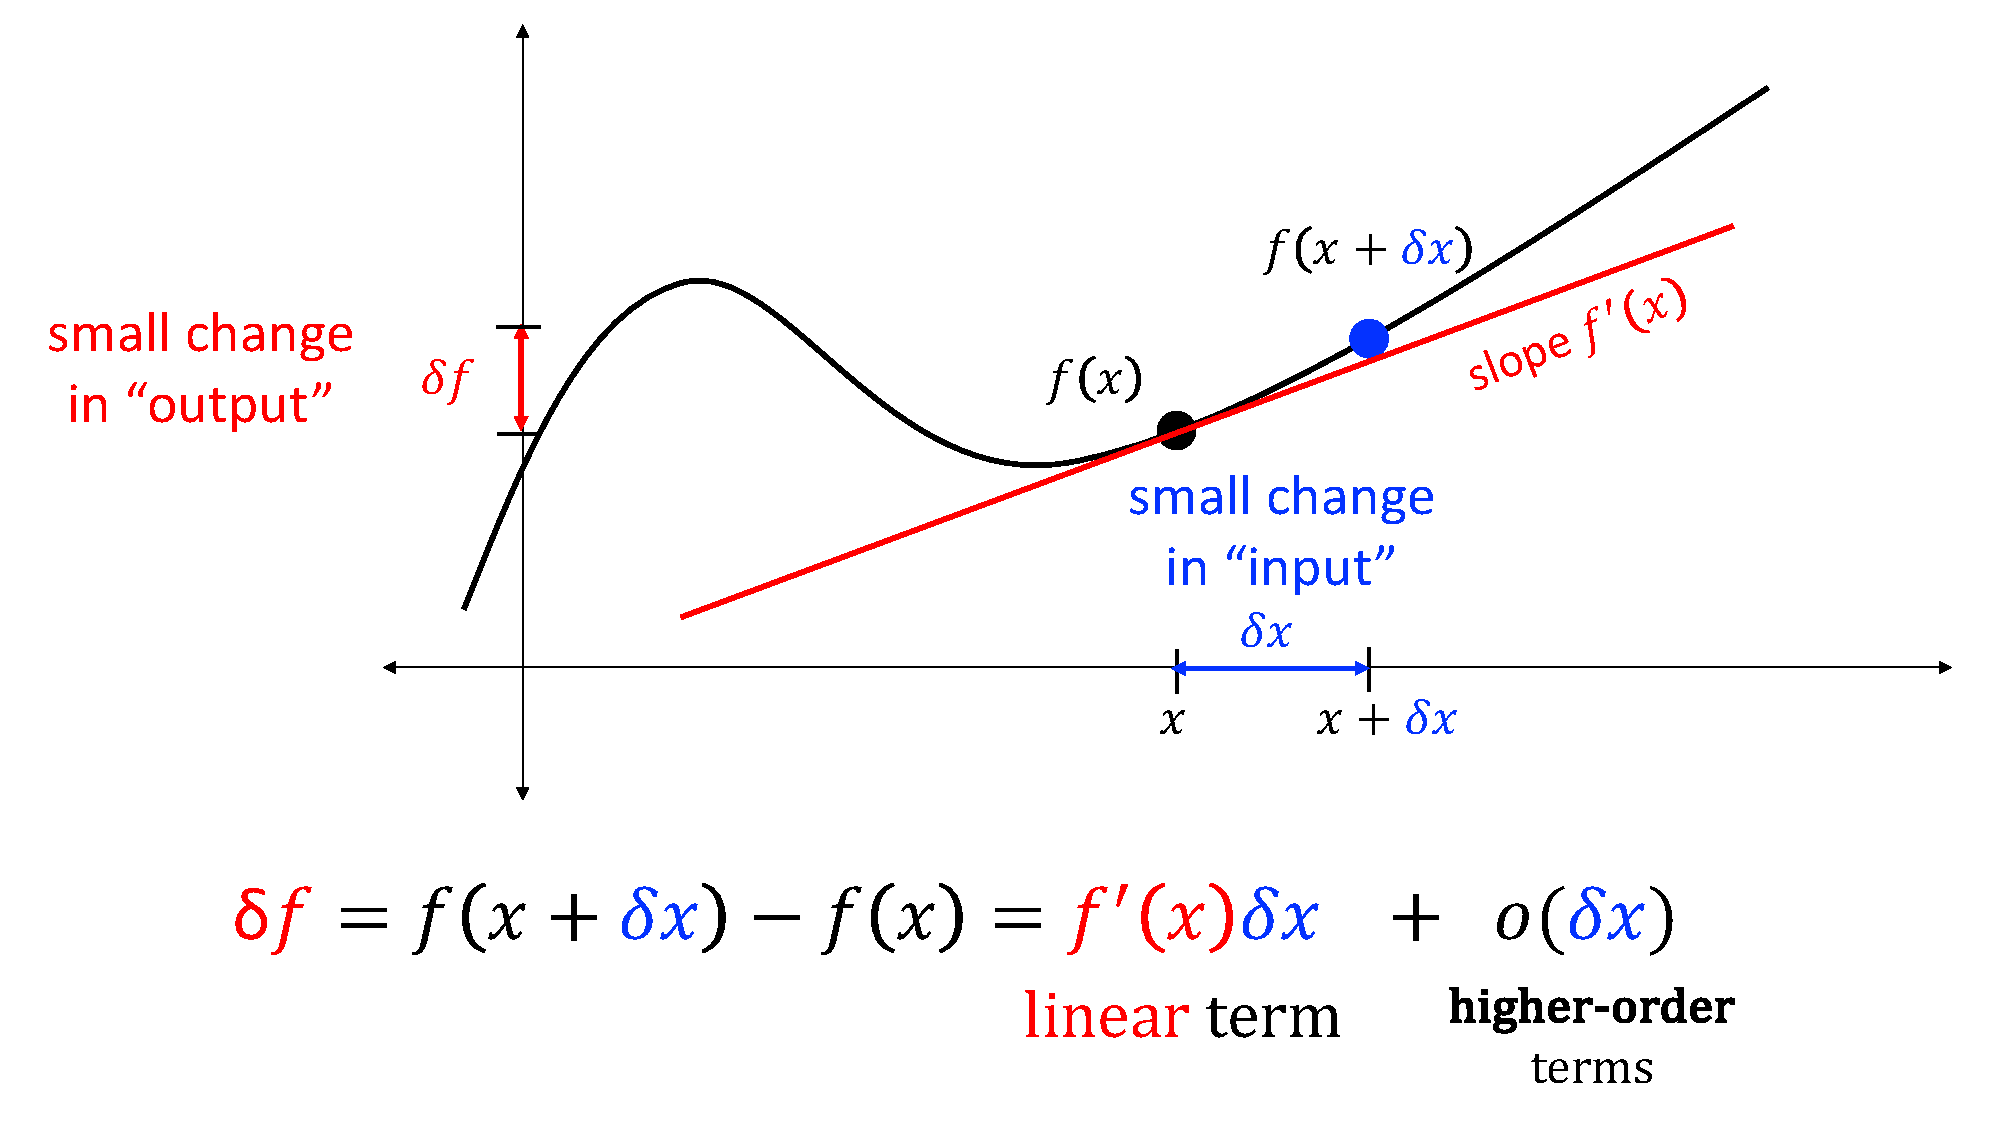
\includegraphics[width=0.8\textwidth]{figures/derivative-linearization.pdf}
    \caption{The essence of a derivative is \emph{linearization}: predicting a small change $\delta f$ in the output $f(x)$ from a small change $\delta x$ in the input $x$, to \emph{first order} in $\delta x$.}
    \label{fig:derivative-linearization}
\end{figure}

In a first-semester single-variable calculus course (like 18.01 at MIT), the derivative $f'(x)$ is  introduced as the slope of the tangent line at the point $(x,f(x))$, which can also be viewed as a \emph{linear approximation} of $f$ near $x$. In particular, as depicted in Fig.~\ref{fig:derivative-linearization}, this is equivalent to a prediction of the \emph{change $\delta f$ in the ``output''} of $f(x)$ from a small \emph{change $\delta x$ in the ``input''} to first order (\emph{linear}) in $\delta x$:
\[
\delta f = f(x+\delta x) - f(x) =  f'(x) \, \delta x  + \underbrace{(\text{higher-order terms})}_{o(\delta x)}.
\]
We can more precisely express these higher-order terms using asymptotic ``little-o'' notation ``$o(\delta x)$'', which denotes any function whose magnitude shrinks much faster than $|\delta x|$ as $\delta x \to 0 $, so that for sufficiently small $\delta x$ it is negligible compared to the linear $f'(x) \, \delta x$ term.  (Variants of this notation are commonly used in computer science, and there is a formal definition that we omit here.\footnote{Briefly, a function $g(\delta x)$ is $o(\delta x)$ if $\lim_{\delta x \to 0} \frac{\Vert g(\delta x) \Vert}{\Vert \delta x \Vert} = 0$.  We will return to this subject in Section~\ref{sec:banach}.})  Examples of such higher-order terms include $(\delta x)^2$, $(\delta x)^3$, $(\delta x)^{1.001}$, and $(\delta x)/\log(\delta x)$.

\begin{remark}
Here, $\delta x$ is \emph{not} an infinitesimal but rather a small number.  Note that our symbol ``$\delta$'' (a Greek lowercase ``delta'') is \emph{not} the same as the symbol ``$\partial$'' commonly used to denote partial derivatives.
\end{remark}

This notion of a derivative may remind you of the first two terms in a Taylor series $f(x+\delta x) = f(x) + f'(x) \, \delta x + \cdots$ (though in fact it is much more basic than Taylor series!), and the notation will generalize nicely to higher dimensions and other vector spaces. In differential notation, we can express the same idea as:
\[
\d f = f(x+\d x) - f(x) = f'(x) \, \d x.
\]
In this notation we implicitly drop the $o(\delta x)$ term that vanishes in the limit as $\delta x$ becomes infinitesimally small.



We will use this as the more generalized definition of a derivative.
 In this formulation, we avoid \emph{dividing} by $\d x$, because soon we will allow $x$ (and hence $\d x$) to be something other than a number---if $\d x$ is a vector, we won't be \emph{able} to divide by it!

\subsection{Linear operators}

From the perspective of linear algebra, given a function $f$, we consider the derivative of $f$, to be the \emph{linear operator} $f'(x)$ such that
\[
\d f = f(x+ \d x) - f(x) = f'(x)[\d x].
\]

As above, you should think of the differential notation $\d x$ as representing an \emph{arbitrary small} change in $x$, where we are implicitly dropping any $o(dx)$ terms, i.e.~terms that decay faster than linearly as $dx\to 0$.  Often, we will omit the square brackets and write simply $f'(x)\d x$ instead of $f'(x)[\d x]$, but this should be understood as the linear operator $f'(x)$ \emph{acting on} $\d x$---don't write $\d x\,f'(x)$, which will generally be nonsense!

This definition will allow us to extend differentiation to \emph{arbitrary vector spaces} of inputs $x$ and outputs $f(x)$.  (More technically, we will require vector spaces with a norm $\Vert x \Vert$, called ``Banach spaces,'' in order to precisely define the $o(\delta x)$ terms that are dropped.  We will come back to the subject of Banach spaces later.)

\begin{recall}[Vector Space]
    Loosely, a vector space (over $\R$) is a set of elements in which addition and subtraction between elements is defined, along with multiplication by real scalars. For instance, while it does not make sense to multiply arbitrary vectors in $\R^n$, we can certainly add them together, and we can certainly scale the vectors by a constant factor.
\end{recall}

Some examples of vector spaces include:
\begin{itemize}
    \item $\R^n$, as described in the above. More generally, $\R^{n\times m}$, the space of $n\times m$ matrices with real entries. Notice again that, if $n\neq m$, then multiplication between elements is not defined.
    \item $C^0(\R^n)$, the set of continuous functions over $\R^n$, with addition defined pointwise.
\end{itemize}

\begin{recall}[Linear Operator]
Recall that a linear operator is a map $L$ from a vector $v$ in vector space $V$ to a vector $L[v]$ (sometimes denoted simply $Lv$) in some other vector space. Specifically, $L$ is linear if
\[
L[v_1+v_2] = Lv_1 + Lv_2 \text{~~and~~} L[\alpha v] = \alpha L[v]
\]
for scalars $\alpha \in \mathbb{R}$.

\textit{Remark}: In this course, $f'$ is a map that takes in an $x$ and spits out a linear operator $f'(x)$ (the \textbf{derivative} of $f$ at $x$). Furthermore, $f'(x)$ is a linear map that takes in an input direction $v$ and gives an output vector $f'(x)[v]$ (which we will later interpret as a directional derivative, see Sec.~\ref{sec:directional}). When the direction $v$ is an infinitesimal $d x$, the output $f'(x)[dx] = df$ is the \textbf{differential} of $f$ (the corresponding infinitesimal change in $f$).
\end{recall}


\begin{notation}[Derivative operators and notations]

There are multiple notations for derivatives in common use, along with multiple related concepts of derivative, differentiation, and differentials.  In the table below, we summarize several of these notations, and put $\boxed{\mathrm{boxes}}$ around the notations adopted for this course:

\vspace{.2cm}

\begin{tabular}{| m{2.1cm} | m{5cm}| m{7cm} |}
\hline
name & notations & remark\tabularnewline
\hline
\hline
derivative
 & $\boxed{f'}$, also $\frac{df}{dx}$, $Df$, $f_{x}$, $\partial_{x}f$,
\dots{} & linear operator $f'(x)$ that maps a small change $dx$ in the input to a small
change ${df=f'(x)[dx]}$ in the output \\
& &
\\
&  & In single-variable calculus, this linear operator can be represented by a \emph{single number}, the ``slope,'' e.g. if $f(x) = \sin(x)$ then $f'(x) = \cos(x)$ is the number that we multiply by $dx$ to get $dy = \cos(x) dx$.  In multi-variable calculus, the linear operator $f'(x)$ can be represented by a \emph{matrix}, the {\bf Jacobian} $J$ (see Sec.~\ref{sec:kronecker}), so that $df = f'(x)[dx] = J\, dx$.  But we will see that it is not always convenient to express $f'$ as a matrix, even if we can.
\tabularnewline
\hline
differentiation & $\boxed{^{\prime}}$, $\frac{d}{dx}$, $D$, \dots{} & linear operator that maps a function $f$ to its derivative $f'$ \tabularnewline
\hline
difference & $\boxed{\delta x}$ and $\boxed{\delta f} = f(x+\delta x) - f(x)$  & small (but \emph{not} infinitesimal) change in the input  $x$ and output $f$ (depending implicitly on $x$ and $\delta x$), respectively:
an element of a vector space, \emph{not} a linear operator\tabularnewline
\hline
differential & $\boxed{d x}$ and $\boxed{d f} = f(x+dx) - f(x)$  & arbitrarily small (``infinitesimal''\footnote{Informally, one can think of the vector space of infinitesimals $\d x$ as living in the same space as $x$  (understood as a small change in a vector, but still a vector nonetheless). Formally, one can define a distinct ``vector space of infinitesimals'' in various ways, e.g.~as a cotangent space in differential geometry, though we won't go into more detail here.} --- we drop higher-order terms) change in the input  $x$ and output $f$, respectively:
an element of a vector space, \emph{not} a linear operator\tabularnewline
\hline
gradient & $\boxed{\nabla f}$ & the vector whose inner product $df = \langle \nabla f, dx \rangle$ with a small change $dx$ in the input gives the small change $df$ in the output.  The ``transpose of the derivative'' $\nabla f = (f')^T$.  (See Sec.~\ref{sec:multivarPart1}.)
\tabularnewline
\hline
partial derivative & $\boxed{\frac{\partial f}{\partial x}}$, $f_{x}$, $\partial_{x}f$ & linear operator that maps a small change $dx$ in a \emph{single argument}
of a multi-argument function to the corresponding change in output,
e.g. for $f(x,y)$ we have $df=\frac{\partial f}{\partial x}[dx]+\frac{\partial f}{\partial y}[dy]$.\tabularnewline
\hline
\end{tabular}
\end{notation}

\newpage

Some examples of linear operators include
\begin{itemize}
    \item Multiplication by scalars $\alpha$, i.e.~$Lv = \alpha v$.  Also  multiplication of column vectors $v$ by matrices $A$, i.e. $Lv = Av$.
    \item Some functions like $f(x)=x^2$ are obviously nonlinear.  But what about $f(x)=x+1$?  This may \emph{look} linear if you plot it, but it is \emph{not} a linear operation, because $f(2x)=2x+1\ne 2f(x)$---such functions, which are linear \emph{plus a nonzero constant}, are known as \emph{affine}.
    \item There are also many other examples of linear operations that are not so convenient or easy to write down as matrix--vector products.  For example, if $A$ is a $3\times 3$ matrix, then $L[A]=AB+CA$ is a linear operator given $3\times 3$ matrices $B,C$.  The transpose $f(x)=x^T$ of a column vector $x$ is linear, but is not given by any matrix multiplied by $x$. Or, if we consider vector spaces of \emph{functions}, then the calculus operations of differentiation and integration are linear operators too!
\end{itemize}

\subsubsection{Directional derivatives}
\label{sec:directional}

There is an equivalent way to interpret this linear-operator viewpoint of a derivative, which you may have seen before in multivariable calculus: as a \textbf{directional derivative}.

If we have a function $f(x)$ of arbitrary vectors $x$, then the directional derivative at $x$ in a direction (vector) $v$ is defined as:
\begin{equation}
\left. \frac{\partial}{\partial \alpha} f(x+\alpha v) \right|_{\alpha = 0} = \lim_{\delta\alpha\to 0} \frac{f(x+\delta\alpha \, v) - f(x)}{\delta \alpha}
\end{equation}
where $\alpha$ is a \emph{scalar}.  This transforms derivatives back into \emph{single-variable calculus} from arbitrary vector spaces.  It measures the rate of change of $f$ in the direction~$v$ from~$x$.  But it turns out that this has a very simple relationship to our linear operator $f'(x)$ from above, because (dropping higher-order terms due to the limit $\delta\alpha \to 0$):
$$
f(x + \underbrace{d\alpha \, v}_{d x}) - f(x) = f'(x)[dx] = d\alpha \, f'(x)[v] \, ,
$$
where we have factored out the scalar $d\alpha$ in the last step thanks to $f'(x)$ being a \emph{linear} operator.  Comparing with above, we immediately find that the directional derivative is:
\begin{equation}
\boxed{ \left. \frac{\partial}{\partial \alpha} f(x+\alpha v) \right|_{\alpha = 0} = f'(x)[v]  }\, .
\end{equation}
It is \emph{exactly equivalent} to our $f'(x)$ from before!   (We can also see this as an instance of the chain rule from Sec.~\ref{sec:chainrule}.) One lesson from this viewpoint is that it is perfectly reasonable to input an arbitrary \emph{non-infinitesimal} vector $v$ into $f'(x)[v]$: the result is not a $df$, but is simply a directional derivative.

\subsection{Revisiting multivariable calculus, Part 1: Scalar-valued functions} \label{sec:multivarPart1}

\begin{figure}
    \centering
    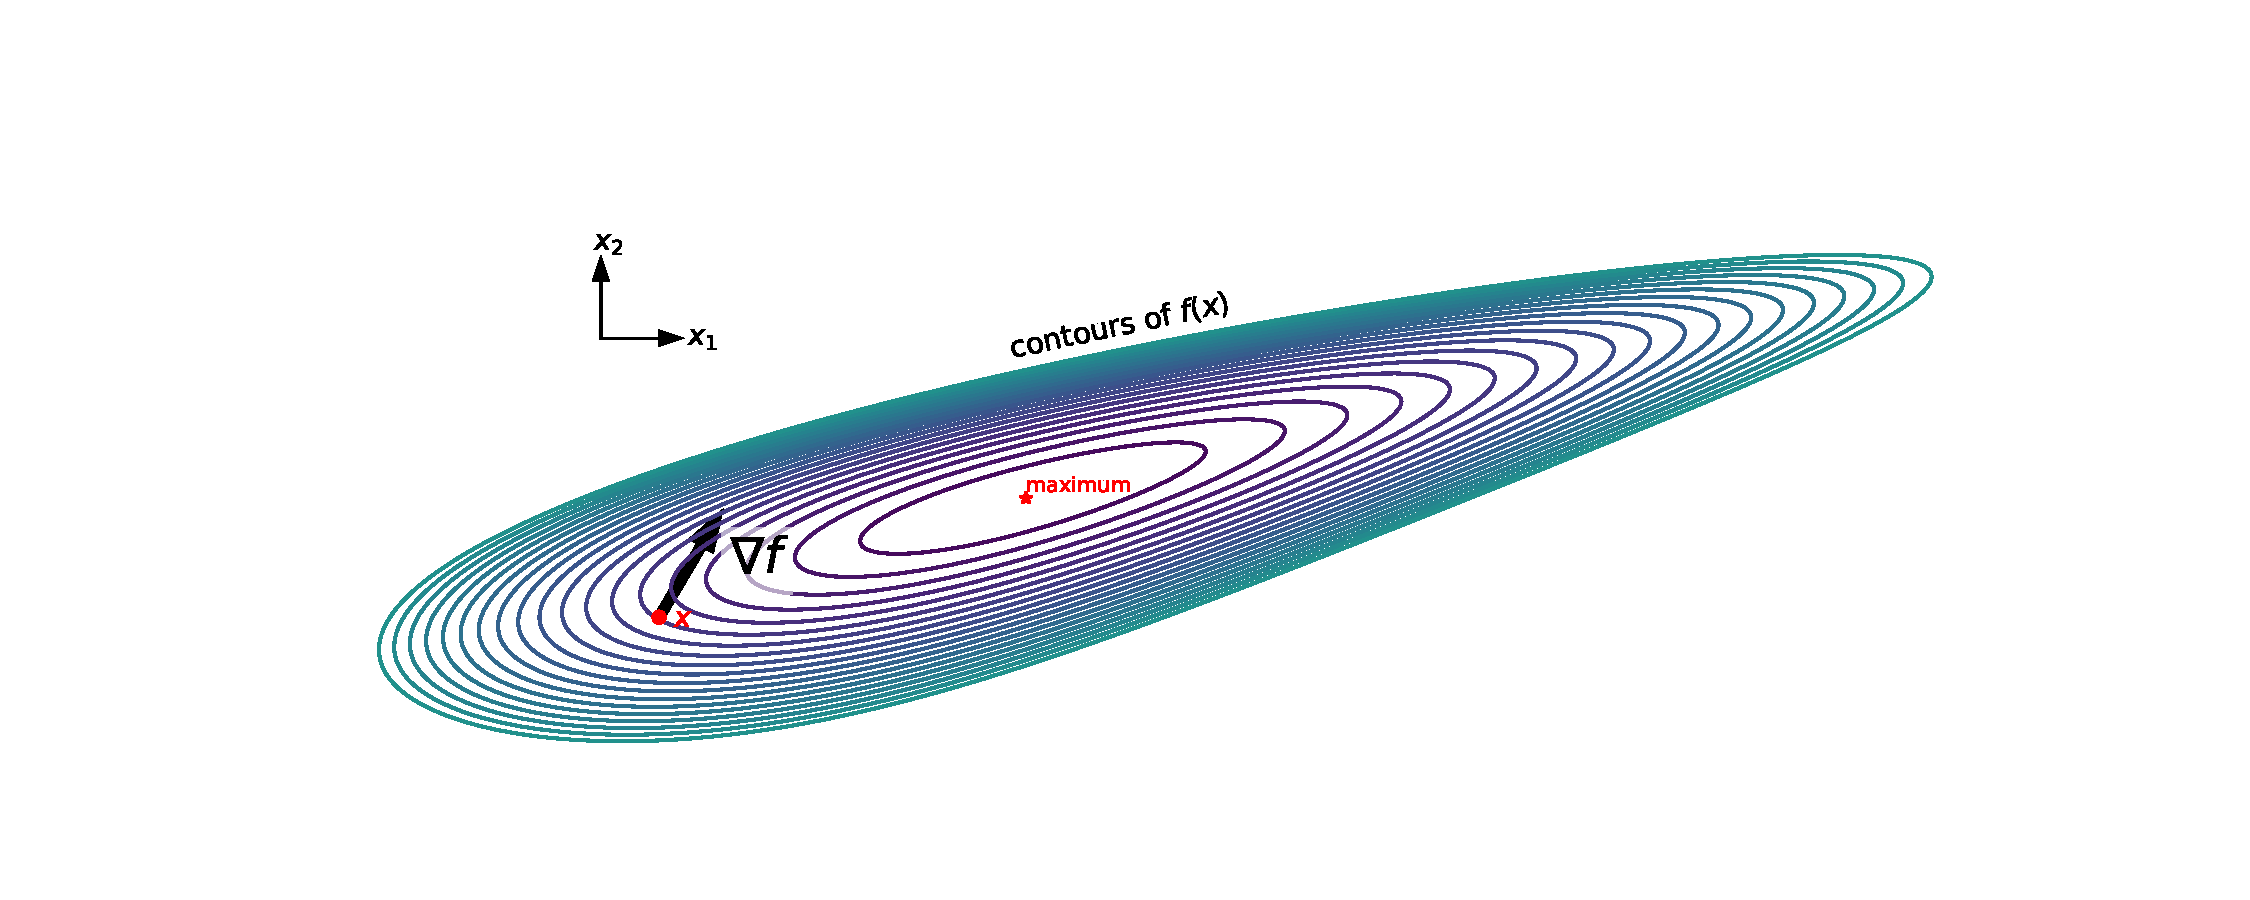
\includegraphics[trim={5cm 2cm 5cm 2cm},clip,width=1.0\textwidth]{figures/gradient-uphill}
    \caption{For a real-valued $f(x)$, the gradient $\nabla f$ is defined so that it corresponds to the ``uphill'' direction at a point $x$, which is perpendicular to the contours of $f$.  Although this may not point exactly towards the nearest local maximum of $f$ (unless the contours are circular), ``going uphill'' is nevertheless the starting point for many computational-optimization algorithms to search for a maximum.}
    \label{fig:gradient-uphill}
\end{figure}

Let $f$ be a scalar-valued function, which takes in ``column'' vectors $x \in \R^n$ and produces a scalar (in $\R$). Then,
\[
\d f = f(x+ \d x) - f(x) = f'(x) [\d x] = \text{scalar}.
\]
Therefore, since $\d x$ is a column vector (in an arbitrary direction, representing an arbitrary small change in $x$), the linear operator $f'(x)$ that produces a scalar $\d f$ must be a \textbf{row vector} (a ``1-row matrix'', or more formally something called a \emph{covector} or ``dual'' vector or ``linear form'')! We call this row vector the \emph{transpose of the gradient} $(\nabla f)^T$, so that $df$ is the \emph{dot (``inner'') product of $dx$ with the gradient}. So we have that
\[
\d f = \nabla f \cdot \d x = \underbrace{(\nabla f)^T}_{f'(x)} \d x \hspace{.25cm} \text{where} \hspace{.25cm} \d x = \begin{pmatrix}
\d x_1 \\  \d x_2 \\ \vdots \\ \d x_n.
\end{pmatrix} .
\]
Some authors view the gradient as a row vector (equating it with $f'$ or the Jacobian), but treating it as a ``column vector'' (the transpose of $f'$), as we do in this course, is a common and useful choice. As a column vector, the gradient can be viewed as the ``uphill'' (\emph{steepest-ascent}) direction in the $x$ space, as depicted in Fig.~\ref{fig:gradient-uphill}.  Furthermore, it is also easier to generalize to scalar functions of other vector spaces. In any case, for this class, we will \textit{always} define $\nabla f$ to \emph{have the same ``shape'' as $x$}, so that $\d f$ is a dot product (``inner product'') of $\d x$ with the gradient.

This is perfectly consistent with the viewpoint of the gradient that you may remember from multivariable calculus, in which the gradient was a vector of components
$$
\nabla f = \begin{pmatrix}
\frac{\partial f}{\partial x_1} \\  \frac{\partial f}{\partial x_2} \\ \vdots \\ \frac{\partial f}{\partial x_n}
\end{pmatrix} \, ;
$$
or, equivalently,
$$
\d f = f(x+\d x)-f(x) = \nabla f \cdot dx = \frac{\partial f}{\partial x_1} dx_1 + \frac{\partial f}{\partial x_2} dx_2 + \cdots + \frac{\partial f}{\partial x_n} dx_n \, .
$$
While a component-wise viewpoint may sometimes be convenient, we want to encourage you to view the vector $x$ as a \emph{whole}, not simply a collection of components, and to learn that it is often more convenient and elegant to differentiate expressions \emph{without} taking the derivative component-by-component, a new approach that will generalize better to more complicated inputs/output vector spaces.

Let's look at an example to see how we compute this differential.

\begin{example}
    Consider $f(x) = x^T Ax$ where $x\in \R^n$ and $A$ is a square $n\times n$ matrix, and thus $f(x) \in \R$. Compute $\d f$, $f'(x)$, and $\nabla f$.
\end{example}

We can do this directly from the definition.
\begin{align*}
    \d f &= f(x+ \d x) - f(x) \\
    &=  (x+ \d x)^T A (x+\d x) - x^T A x \\
    &= \cancel{x^T A x} + \d x^T\, Ax + x^T A \d x + \cancelto{\text{higher order}}{\d x^T \,A \d x} - \cancel{x^T A x} \\
    &= \underbrace{x^T(A+A^T)}_{f'(x)=(\nabla f)^T }\d x \implies \nabla f = (A+A^T)x \, .
\end{align*}
Here, we dropped terms with more than one $\d x$ factor as these are asymptotically negligible.  Another trick was to combine $\d x^T A x$ and $x^T A \d x$ by realizing that these are \emph{scalars} and hence equal to their own transpose: $dx^T A x = (\d x^T A x)^T = x^T A^T \d x$. Hence, we have found that $f'(x) = x^T(A+A^T) = (\nabla f)^T$, or equivalently $\nabla f = [x^T(A+A^T)]^T = (A+A^T)x$.

It is, of course, also possible to compute the same gradient component-by-component, the way you probably learned to do in multivariable calculus.  First, you would need to write $f(x)$ explicitly in terms of the components of $x$, as $f(x) = x^T A x = \sum_{i,j} x_i A_{i,j} x_j$.  Then, you would compute $\partial f/\partial x_k$ for each $k$, taking care that $x$ appears twice in the $f$ summation.  However, this approach is awkward, error-prone, labor-intensive, and quickly becomes worse as we move on to more complicated functions.  It is much better, we feel, to get used to treating vectors and matrices \emph{as a whole}, not as mere collections of numbers.

\subsection{Revisiting multivariable calculus, Part 2: Vector-valued functions}

Next time, we will revisit multi-variable calculus (18.02 at MIT) again in a Part 2, where now $f$ will be a vector-valued function, taking in vectors $x\in \R^n$ and giving vector outputs $f(x) \in \R^m$. Then, $\d f$ will be a $m$-component column vector, $\d x$ will be an $n$-component column vector, and we must get a linear operator $f'(x)$ satisfying
\[
\underbrace{\d f}_{m\text{ components}} = \underbrace{f'(x)}_{m \times n} \underbrace{\d x}_{n\text{ components}} \, ,
\]
so $f'(x)$ must be an $m \times n$ \emph{matrix} called the \textit{Jacobian} of $f$!

The Jacobian matrix $J$
represents the linear operator that takes $dx$ to $df$:
\[
\d f = J \d x \, .
\]
The matrix $J$ has entries $J_{ij}=\frac{\partial f_i}{\partial x_j}$ (corresponding to the $i$-th row and the $j$-th column of $J$).

So now, suppose that $f: \R^2 \to \R^2$. Let's understand how we would compute the differential of $f$:
\[
\d f = \begin{pmatrix}
   \frac{\partial f_1}{\partial x_1} & \frac{\partial f_1}{\partial x_2} \\ \frac{\partial f_2}{\partial x_1} & \frac{\partial f_2}{\partial x_2}
\end{pmatrix} \begin{pmatrix}
     \d x_1 \\ \d x_2
\end{pmatrix} = \begin{pmatrix}
    \frac{\partial f_1}{\partial x_1}\d x_1 +  \frac{\partial f_1}{\partial x_2}\d x_2 \\ \frac{\partial f_2}{\partial x_1}\d x_1 +  \frac{\partial f_2}{\partial x_2} \d x_2
\end{pmatrix}.
\]

Let's compute an example.
\begin{example}\label{ex1}
    Consider the function $f(x) = Ax$ where $A$ is a constant $m\times n$ matrix. Then, by applying the distributive law for matrix--vector products, we have
\begin{align*}
    \d f &= f(x+\d x ) - f(x) =  A(x + \d x) - Ax  \\
    &= \cancel{Ax} + A\d x - \cancel{Ax} = A\d x = f'(x) \d x.
\end{align*}
Therefore, $f'(x) = A$.
\end{example}

Notice then that the linear operator $A$ is its own Jacobian matrix!

Let's now consider some derivative rules.

\begin{itemize}
    \item \textbf{Sum Rule}: Given $f(x) = g(x) + h(x)$, we get that
    \[
\d f = \d g + \d h \implies f'(x) \d x = g'(x) \d x + h'(x)\d x.
    \]
    Hence, $f' = g'+h'$ as we should expect.  This is the linear operator $f'(x)[v] = g'(x)[v] + h'(x)[v]$, and note that we can sum linear operators (like $g'$ and $h'$) just like we can sum matrices! In this way, linear operators form a vector space.
    \item \textbf{Product Rule}: Suppose $f(x) = g(x) h(x)$. Then,
    \begin{align*}
        \d f &= f(x+ \d x) - f(x) \\
        &= g(x+\d x) h(x+\d x) - g(x) h(x) \\
        &= (g(x) + \underbrace{g'(x) \d x}_{\d g}) (h(x) + \underbrace{h'(x)\d x}_{\d h}) - g(x)h(x) \\
        &= g h + dg\, h + g\,dh + \cancelto{0}{dg \,dh} - gh \\
        &= \d g \, h + g \,\d h \, ,
    \end{align*}
    where the $\d g \, \d h$ term is higher-order and hence dropped in infinitesimal notation.
    Note, as usual, that $\d g$ and $h$ may not commute now as they may no longer be scalars!
\end{itemize}

Let's look at some short examples of how we can apply the product rule nicely.

\begin{example}\label{ex:Ax}
    Let $f(x) = Ax$ (mapping $\R^n \to \R^m$) where $A$ is a constant $m\times n$ matrix. Then,
    \[
    \d f = d(Ax) =  \cancelto{0}{\d A} \, x + A\d x = A\d x \implies f'(x) = A.
    \]
    We have ${\d A} = 0$ here because $A$ does not change when we change $x$.
\end{example}

\begin{example}
    Let $f(x) = x^T A x$ (mapping $\R^n \to \R$). Then,
    \[
    \d f = \d x^T(Ax) + x^T \d(Ax) = \underbrace{\d x^T \, Ax}_{=\, x^T A^T\d x} + x^T A\d x = x^T(A+A^T)\d x  = (\nabla f)^T \d x\, ,
    \]
    and hence $f'(x) = x^T(A + A^T)$. (In the common case where $A$ is symmetric, this simplifies to $f'(x) = 2x^T A$.) Note that here we have applied Example~\ref{ex:Ax} in computing $d(Ax) = A dx$.
    Furthermore, $f$ is a scalar valued function, so we may also obtain the gradient $\nabla f = (A+A^T) x$ as before (which simplifies to $2Ax$ if $A$ is symmetric).
\end{example}

\begin{example}[Elementwise Products]
    Given $x,y\in \R^m$, define
    $$x\dotstar y = \begin{pmatrix}
        x_1y_1 \\ \vdots \\ x_my_m
    \end{pmatrix} = \underbrace{\begin{pmatrix} x_1 & & & \\ & x_2 & & \\ & & \ddots & \\ & & & x_m \end{pmatrix}}_{\mathrm{diag}(x)} \begin{pmatrix}
        y_1 \\ \vdots \\ y_m
    \end{pmatrix},$$
    the element-wise product of vectors (also called the \href{https://en.wikipedia.org/wiki/Hadamard_product_(matrices)}{Hadamard product}), where for convenience below we also define $\mathrm{diag}(x)$ as the $m \times m$ diagonal matrix with $x$ on the diagonal. Then, given $A \in \R^{m,n}$, define $f:\R^n \to \R^m$ via
    \[
    f(x) = A(x\dotstar x).
    \]

    As an exercise, one can verify the following:
    \begin{itemize}
        \item[(a)] $x\dotstar y = y\dotstar x$,
        \item[(b)] $A(x\dotstar y) = A \, \mathrm{diag}(x)\, y$.
        \item[(c)] $d(x\dotstar y) = (\d x)\dotstar y + x\dotstar(\d y)$.  So if we take $y$ to be a constant and define $g(x) = y \dotstar x$, its Jacobian matrix is $\mathrm{diag}(y)$.
        \item[(d)] $\d f = A(2x\dotstar dx) = 2A \, \mathrm{diag}(x) \, dx = f'(x)[dx]$, so the Jacobian matrix is $J = 2A \, \mathrm{diag}(x)$.
        \item[(e)] Notice that the directional derivative (Sec.~\ref{sec:directional}) of $f$ at $x$ in the direction $v$ is simply given by $f'(x)[v] = 2A (x \dotstar v)$.   One could also check numerically for some arbitrary $A,x,v$ that $f(x + 10^{-8} v) - f(x) \approx 10^{-8} ( 2A (x \dotstar v))$.
    \end{itemize}
\end{example}

\subsection{The Chain Rule}
\label{sec:chainrule}

One of the most important rules from differential calculus is the chain rule, because it allows us to differentiate complicated functions built out of compositions of simpler functions.   This chain rule can also be generalized to our differential notation in order to work for functions on arbitrary vector spaces:
\begin{itemize}
    \item \textbf{Chain Rule}: Let $f(x) = g(h(x))$. Then,
    \begin{align*}
    \d f = f(x + \d x) - f(x) &= g(h( x + \d x)) - g(h(x)) \\
    &= g'(h(x))[h(x + \d x) - h(x)] \\
    &= g'(h(x))[h'(x)[\d x]] \\
    &= g'(h(x)) h'(x) [\d x]
    \end{align*}
    where $g'(h(x))h'(x)$ is a composition of $g'$ and $h'$ as matrices.

    In other words, $f'(x) = g'(h(x)) h'(x)$: the Jacobian (linear operator) $f'$ is simply the \emph{product (composition) of the Jacobians}, $g' h'$.  Ordering matters because linear operators do not generally commute: left-to-right = outputs-to-inputs.
\end{itemize}

Let's look more carefully at the \emph{shapes} of these Jacobian matrices in an example where each function maps a column vector to a column vector:
\begin{example}
    Let $x\in \R^n$, $h(x) \in \R^p$, and $g(h(x)) \in \R^m$. Then, let $f(x) = g(h(x))$ mapping from $\R^n$ to $\R^m$. The chain rule then states that
    \[
    f'(x) = g'(h(x)) h'(x),
    \]
    which makes sense as $g'$ is an $m\times p$ matrix and $h'$ is a $p\times n$ matrix, so that the product gives an $m \times n$ matrix $f'$! However, notice that this is \textit{not} the same as $h'(x) g'(h(x))$ as you cannot (if $n\neq m$) multiply a $p\times n$ and an $m\times p$ matrix together, and even if $n = m$ you will get the wrong answer since they probably won't commute.
\end{example}

Not only does the order of the multiplication matter, but the associativity of matrix multiplication matters \textit{practically}. Let's consider a function
\[
f(x)= a(b(c(x)))
\]
where $c: \R^n \to \R^p$, $b:\R^p \to \R^q$, and $a: \R^q\to \R^m$. Then, we have that, by the chain rule,
\[
f'(x) = a'(b(c(x))) b'(c(x))c'(x).
\]
Notice that this is the same as
\[
f'  = (a' b')c' = a'(b'c')
\]
by associativity (omitting the function arguments for brevity). The left-hand side is multiplication from left to right, and the right-hand side is multiplication from right to left.

But who cares? Well it turns out that associativity is deeply important. So important that the two orderings have names: multiplying  left-to-right is called ``reverse mode''  and multiplying right-to-left is called ``forward mode'' in the field of \textit{automatic differentiation} (AD).  Reverse-mode differentation is also known as an ``adjoint method'' or ``backpropagation'' in some contexts, which we will explore in more detail later. Why does this matter? Let's think about the computational cost of matrix multiplication.


\subsubsection{Cost of Matrix Multiplication}
\label{sec:cost-matrix-mult}

\begin{figure}
    \centering
    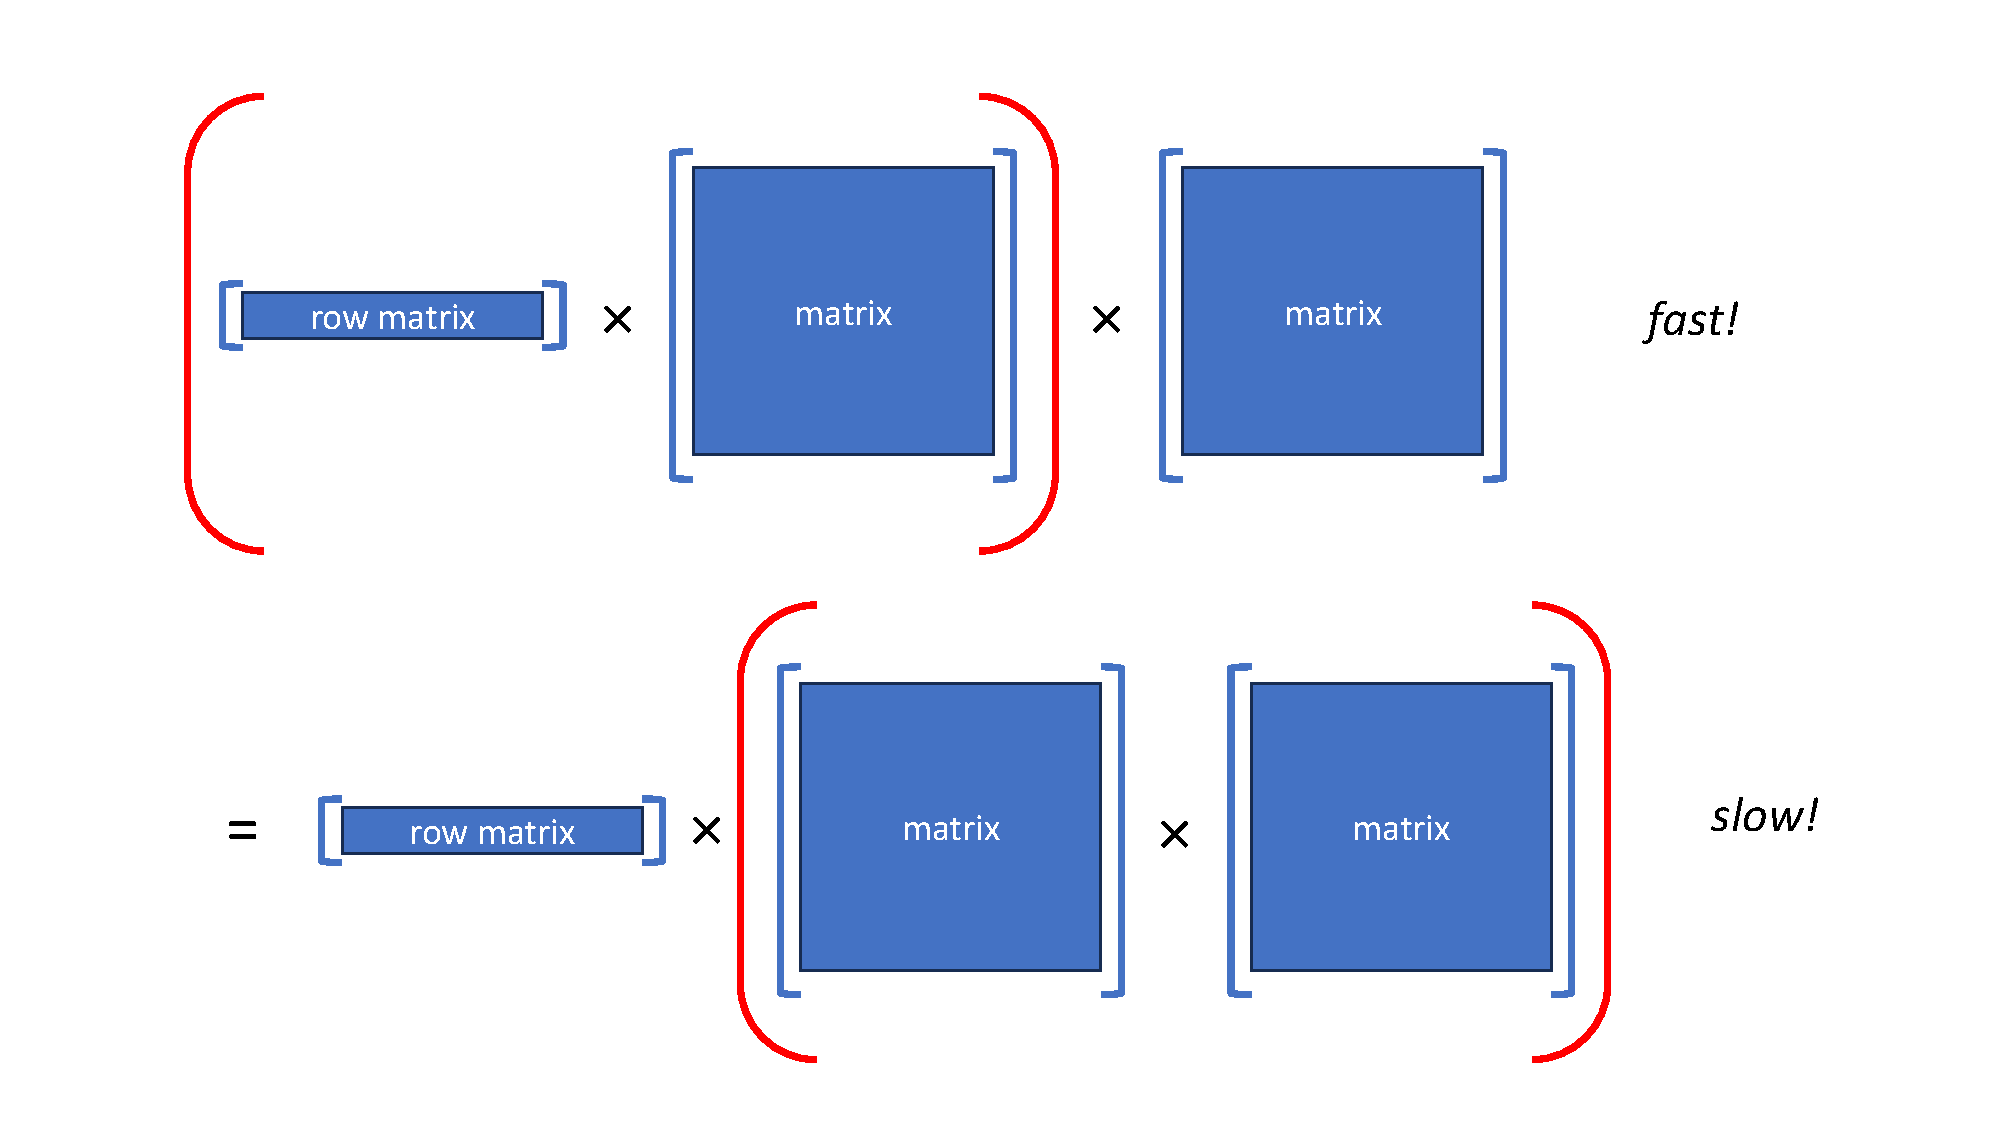
\includegraphics[width=0.8\textwidth]{figures/matrix-mult-assoc}
    \caption{Matrix multiplication is \emph{associative}---that is, $(AB)C = A(BC)$ for all $A,B,C$---but multiplying left-to-right can be much more efficient than right-to-left if the leftmost matrix has only one (or few) rows, as shown here.  Correspondingly, the order in which you carry out the chain rule has dramatic consequences for the computational effort required.  Left-to-right is known as ``reverse mode'' or ``backpropagation'', and is best suited to situations where there are many fewer outputs than inputs.}
    \label{fig:matrix-mult-assoc}
\end{figure}

If you multiply a $m\times q$ matrix by a $q\times p$ matrix, you normally do it by computing $mp$ dot products of length $q$ (or some equivalent re-ordering of these operations). To do a dot product of length $q$ requires $q$ multiplications and $q-1$ additions of scalars. Overall, this is approximately $2mpq$ scalar operations in total. In computer science, you would write that this is ``$\Theta(mpq)$'': the computational effort is \emph{asymptotically proportional} to $mpq$ for large $m,p,q$.

So why does the order of the chain rule matter? Consider the following two examples.
\begin{example}
    Suppose you have a lot of inputs $n \gg 1$, and only one output $m=1$, with lots of intermediate values, i.e. $q=p=n$. Then reverse mode (left-to-right) will cost $\Theta(n^2)$ scalar operations while forward mode (right-to-left) would cost $\Theta(n^3)$! This is a huge cost difference, depicted schematically in Fig.~\ref{fig:matrix-mult-assoc}.

    Conversely, suppose you have a lot of outputs $m \gg 1$ and only one input $n=1$, with lots of intermediate values $q=p=m$.  Then reverse mode would cost $\Theta(m^3)$ operations but forward mode would be only $\Theta(m^2)$!

    Moral: If you have a lot of inputs and few outputs (the usual case in machine learning and optimization), compute the chain rule left-to-right (reverse mode).  If you have a lot of outputs and few inputs, compute the chain rule right-to-left (forward mode).  We return to this in Sec.~\ref{sec:forward-vs-reverse}.
\end{example}

\subsection{Beyond Multi-Variable Derivatives}

Now let's compute some derivatives that go beyond first-year calculus, where the inputs and outputs are in more general vector spaces. For instance, consider the following examples:

\begin{example}
    Let $A$ be an $n\times n$ matrix. You could have the following matrix-valued functions. For example:
\begin{itemize}
    \item $f(A) = A^3$,
    \item $f(A) = A^{-1}$ if $A$ is invertible,
    \item or $U$, where $U$ is the resulting matrix after applying Gaussian elimination to $A$!
\end{itemize}

\noindent You could also have scalar outputs. For example:
\begin{itemize}
    \item $f(A) = \det A$,
    \item $f(A) =$ trace $A$,
    \item or $f(A) = \sigma_1(A)$, the largest singular value of $A$.
\end{itemize}
\end{example}

Let's focus on two simpler examples for this lecture.
\begin{example}
    Let $f(A) = A^3$ where $A$ is a square matrix. Compute $\d f$.
\end{example}

Here, we apply the chain rule one step at a time:
\[
\d f = \d A\, A^2 + A \,\d A \, A + A^2 \,\d A = f'(A) [\d A].
\]
Notice that this is not equal to $3A^2$ (unless $\d A$ and $A$ commute, which won't generally be true since $\d A$ represents an \emph{arbitrary} small change in $A$).   The right-hand side is a linear operator $f'(A)$ acting on $\d A$, but it is not so easy to interpret it as simply a single ``Jacobian'' matrix multiplying $\d A$!

\begin{example}
    Let $f(A) = A^{-1}$ where $A$ is a square invertible matrix. Compute $\d f = \d(A^{-1})$.
\end{example}

Here, we use a slight trick. Notice that $AA^{-1} = \Id$, the identity matrix. Thus, we can compute the differential using the product rule (noting that $\d\Id = 0$, since changing $A$ does not change $\Id$) so
\[
\d(AA^{-1}) = \d A\, A^{-1} + A\,\d(A^{-1}) = \d (\Id) = 0\implies \d(A^{-1}) = -A^{-1} \,\d A \,A^{-1}.
\]
